\title{Использование символьных конечных преобразователей для лексического анализа динамически формируемого кода}

\titlerunning{Использование символьных конечных преобразователей для лексического анализа динамически формируемого кода}

\author{Гумин Егор Дмитриевич}

\authorrunning{Е.Д.Гумин}

\tocauthor{Е.Д.Гумин}
\institute{Санкт-Петербургский государственный университет\\
\email{gumin.egor@gmail.com}}

\maketitle             

\begin{abstract}
При статическом анализе динамически формируемого кода возникает необходимость применения лексического анализа к нелинейному входному потоку.
Для решения этой задачи в проекте YaccConstructor используется композиция конечных преобразователей, 
представляющих входной поток и лексер целевого языка, 
однако существующая реализация обладает недостаточной производительностью. 
Целью данной работы является исследование возможности увеличения производительности лексического анализа динамического кода
 за счет применения библиотеки Microsoft.Automata, 
специализированной для работы с преобразователями.
\end{abstract}

\section*{Введение}

Синтаксический анализ, как правило, используется для построения структурного представления кода с использованием грамматики, описывающей разбираемый язык. Абстрактное синтаксическое дерево, являющееся результатом работы синтаксического анализатора, в дальнейшем используется для проведения статического анализа кода или же в каких-то других целях. Как правило, на вход синтаксическому анализатору подаётся линейная последовательность токенов, представляющая код программы. Однако могут возникать ситуации, когда вход не может быть представлен линейно. Такие ситуации могут возникать, например, при автоматической генерации кода. Генерация может происходить в циклах, с использованием условных операторов или строковых операций. Поэтому для описания генерируемых цепочек можно использовать конечный автомат, порождающий цепочки, который уже не будет являться линейным. Такую задачу будем называть синтаксическим анализом регулярных множеств.

Кроме этого, ещё одной областью, где может быть применим синтаксический анализ регулярных множеств, является бионформатика. Одной из часто возникающих задач в биоинформатике является классификация организмов, находящихся в образцах, полученных из окружающей среды~\cite{bioRNA}. По образцам строится метагеномная сборка, которая содержит в себе смесь из ДНК всех содержащихся в сборке организмов. В свою очередь ДНК является последовательностью символов в алфавите \{A, C, G, T\}. ДНК организмов, которые относятся к одному и тому же виду, содержат одинаковые подцепочки, которые и необходимо выделить, чтобы классифицировать организм. Как правило, эти подцепочки~--- это последовательности РНК. РНК может быть описана с помощью грамматики. Метагеномная сборка, в свою очередь, может быть представлена в виде графа с цепочками на рёбрах. Таким образом, в таком графе необходимо найти цепочки, выводимые в грамматике, описывающей РНК. 

Грамматики, описывающие структуру РНК, являются неоднозначными. Грамматика называется неоднозначной, если одна и та же цепочка может быть выведена несколькими способами. Такие алгоритмы синтаксического анализа как LR и LL не позволяют обрабатывать неоднозначные грамматики. Для работы с неоднозначными грамматиками существуют алгоритмы обобщённого синтаксического анализа GLR~\cite{GLR}, GLL~\cite{GLL}. В рамках проекта YaccConstructor~\cite{YaccConstructorPage, YaccConstructorPaper} был реализован алгоритм GLL, кроме того, была предложена его модификация для обработки нелинейных входных данных~--- графов. Реализованная модификация позволяет находить цепочки транспортной РНК (тРНК) в небольших метагеномных сборках, возвращая координаты начала и конца найденной цепочки. Проблема заключается в том, что грамматика для описания тРНК является сильно неоднозначной, что сказывается на производительности и точности полученных результатов. Для повышения точности можно применять конъюнктивные грамматики~\cite{ConjGrammars}, в которых для описания продукций используется операция конъюнкции. Такие грамматики расширяют класс контекстно-свободных языков и позволяют точнее описать структуру тРНК. Данная работа посвящена описанию модификаций решения на основе алгоритма GLL для работы с конъюнктивными грамматиками.

\section{Постановка задачи}
Целью данной работы является исследование применимости символьных конечных преобразователей для лексического анализа. Для ее достижения поставлены следующие задачи:

\begin{itemize}
    \item Изучить возможности библиотеки Microsoft.Automata.
\item Провести сравнение производительности алгоритма операции композиции над символьными конечными преобразователями в библиотеке Microsoft.Automata с производительностью операции композиции над конечными преобразователями в исследовательском проекте YaccConstructor.
\item На основании полученных результатов сделать выводы о применимости библиотеки Microsoft.Automata для лексического анализа в проекте YaccConstructor.
  \end{itemize}

\section{Обзор}
\lstset{basicstyle=\normalsize\ttfamily, columns=fullflexible}
В данном обзоре рассматриваются некоторые подходы к заданию принтеров и форматеров, а также плагин Grammar-Kit для IntelliJ IDEA, позволяющий по БНФ-грамматике задавать синтаксический анализатор целевого языка.
Используемые плагином грамматики рассматриваются на примере грамматики языка While \cite{paper:nielson}.

\subsection{Подходы к заданию принтеров и форматеров}
Рассмотрим некоторые подходы к заданию принтеров и форматеров.
\subsubsection{Задание форматеров по описанию синтаксиса}%Язык описания синтаксиса}
Существуют различные подходы к заданию принтеров для целевого языка.
Один из них описан в \cite{paper:tbe}.
Авторы предлагают язык описания синтаксиса, по которому можно получить и синтаксический анализатор, и принтер для языка.
Описание синтаксиса состоит из правил, которые схожи с правилами формальных грамматик, но которые также задают и стиль форматирования для данной структуры языка.
Приведенное ниже правило вывода описывает основные арифметические выражения:
{
    \lstinputlisting{codes/tbeif.txt}
    %% =================================================
    %% ПРИМЕР ПОИНТЕРЕСНЕЕ
    %% непонятно, как задаются условия форматирования
    %% =================================================
}
\noindent
Первое преобразование определяет шаблон для выражений, состоящих из чисел.
Остальные преобразования задают шаблоны для операций сложения и вычитания.
Каждое из них состоит из двух меток \lstinline{<Exp>} для подстановки выражений, арифметического знака, а также двух пробелов вокруг этого знака.
Само правило явно задает способ, которым будут отформатированы арифметические выражения полученного языка.
%При дальнейшем форматировании программ на данном языке, арифметические выражения будут иметь вид, задаваемый правилом.
Вместо пробелов можно также указать табуляции и/или переносы строк.
Недостатком данного подхода является то, что правила форматирования задаются заранее, и, чтобы их изменить, необходимо менять описание синтаксиса языка.
Кроме того, каждое такое правило задает единственный вариант форматирования данной структуры.

%\subsubsection{}
Наиболее близкий к нашей работе метод описан в \cite{paper:asf-sdf}.
Принтер языка может быть получен по ASF+SDF описанию языка \cite{paper:klint}, что представляет собой контекстно-свободную грамматику.
При этом правила форматирования не указываются.
Недостатком данного подхода является то, что при генерации принтера задается базовый стиль форматирования, и, чтобы его изменить, необходимо редактировать сгенерированный код, тогда как подход с использованием синтаксических шаблонов позволяет пользователю декларативным образом настраивать принтер.

\subsubsection{Форматеры, встроенные в IDE}
Так же широко распространены форматеры, встроенные в IDE.
Они используют множество настроек для задания стиля форматирования (рис.~\ref{ov:settings}).
Среди них: тип и размер отступов, расположение фигурных скобок в C-подобных языках, политика переноса списочных выражений на новую строку и десятки других.
Набор этих настроек выбирается разработчиком форматера на основе его представлений о возможных стилях кодирования для целевого языка.
Такие форматеры обычно тесно интегрированы с IDE, имеют высокую скорость работы, и их выразительности, как правило, достаточно для задания необходимого стиля форматирования.
Однако для поддержки нового языка необходимо определить нужный набор настроек и вручную реализовать форматер.
В случае, если пользователю необходимо придерживаться стиля кодирования некоторой существующей кодовой базы, то ему нужно самостоятельно определить значения этих настроек.
Данный недостаток отсутствует в работе \cite{paper:sformatters}, где авторы предлагают инструмент, позволяющий получить некоторые настройки форматера из существующего программного кода.
Недостатком подхода является то, что число этих настроек невелико: система позволяет определять только стиль отступов, стили именования идентификаторов, необходимое количество комментариев.
Другой подход \cite{blog:genformat} предлагает использование генетического алгоритма 
%\footnote{\texttt{https://en.wikipedia.org/wiki/Genetic\textunderscore algorithm}} 
для поиска настроек форматера в исходном коде программ на языке C.

%и в работе\footnote{\texttt{https://blog.jetbrains.com/clion/2015/11/applying-genetic-algorithms-to-automatic-code-formatting/}}. 
%Они представляют собой способы автоматического вычленения настроек форматирования из программного кода.
\begin{figure}[t]
    \centering
    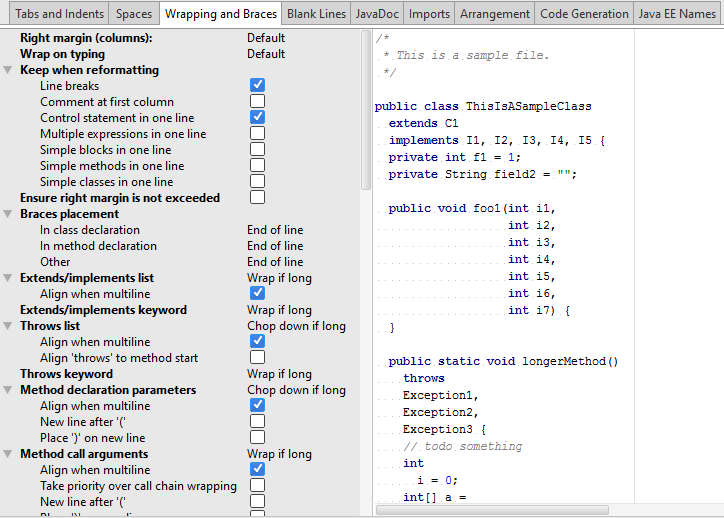
\includegraphics[width=.7\textwidth]{images/settingsjava.PNG}
    \caption{Настройки форматера языка Java в IntelliJ IDEA}
    \label{ov:settings}
\end{figure}

\subsection{Grammar-Kit}
Как уже было отмечено, для поддержки нового языка в платформе IntelliJ IDEA необходимо разработать синтаксический анализатор.
Для его генерации можно использовать плагин Grammar-Kit.
В качестве системы описания синтаксиса языка используется БНФ-грамматика.
Результатом работы плагина является код синтаксического анализатора и иерархия классов внутреннего представления. %(для IntelliJ IDEA~--- \emph{PSI-классов}).%PSI-классов.
%PSI-классом является каждая структура языка, вместе они образуют иерархию.

%Кроме того, при реализации поддержки нового языка в платформе возникает потребность в форматере.
%Мы хотим задавать принтер для языка, используя его грамматику.
% что тут еще описывать?
%\subsection{Грамматика языка While}
%Для апробации метода, описанного в \cite{paper:while}, использовался язык While, поэтому будем рассматривать грамматики, с которыми работает Grammar-Kit, на примере грамматики языка While.
Рассмотрим грамматику языка While, для которого производилась апробация метода, описанного в \cite{paper:while}.
%Рассмотрим БНФ-грамматику, использующуюся в плагине Grammar-Kit на примере грамматики языка While (рис.~\ref{ov:whileBnfFull}).
%\begin{figure}[p]
%\fvset{frame=lines,framesep=5pt}
While~--- язык программирования, содержащий следующие конструкции: чтение из стандартного потока (\lstinline{read}) и запись в стандартный поток (\lstinline{write}), оператор ветвления (\lstinline{if}), цикл с предусловием (\lstinline{while}); процедуры (\lstinline{proc}), бинарные выражения (\lstinline{binary_expr}), в том числе булевы (\lstinline{binary_bexpr}) и т. д.
% (рис.~\ref{ov:whileI},~\ref{ov:whileII},~\ref{ov:whileIII}).
\begin{figure}[h]
 %   \begin{pyglist}[numbers=left,numbersep=5pt]%, basicstyle=\ttfamily]
    \begin{lstlisting}[numbers=left, numbersep=3pt, basicstyle=\ttfamily\small, numberstyle=\tiny, frame=bottom, language={}]
whileFile  ::= proc_list stmt_list
stmt_list  ::= stmt*
proc_list  ::= procedure*
stmt       ::= skip|assign|if|while|write|read
skip       ::= 'skip' ';'
write      ::= 'write' '(' expr ')' ';'
read       ::= 'read' '(' id ')' ';'
assign     ::= id ':=' expr ';'
if         ::= 'if' '(' bexpr ')' 'then' stmt_list ('else' stmt_list)? 'fi'
while      ::= 'while' '(' bexpr ')' 'do' stmt_list 'od'
procedure  ::= 'proc' id '(' param_list ')' stmt_list 'endp'
param_list ::= ref_expr? (',' ref_expr)*
...
 \end{lstlisting}
    \caption{Грамматики языка While. Операторы языка}
    \label{ov:whileI}
\end{figure}
\noindent
На рис.~\ref{ov:whileI} представлена часть грамматики языка While, задающая множество операторов.
Рассмотрим правило грамматики, задающее оператор ветвления.
Правая часть правила состоит из терминалов \lstinline{'if'}, \lstinline{'then'} \lstinline{'('} и др.; нетерминалов: \lstinline{bexpr}, \lstinline{stmt_list}, а также условного вхождения \lstinline{('else' stmt_list)?} (то есть конструкция может отсутствовать в программах на данном языке).
Некоторые правила грамматики имеют модификаторы, которые используются для дополнительных указаний генератору синтаксического анализатора (рис.~\ref{ov:whileII}).
\begin{figure}[h]
    %\begin{pyglist}[numbers=left,numbersep=5pt]
    \begin{lstlisting}[numbers=left, numbersep=3pt, basicstyle=\ttfamily\small, numberstyle=\tiny, frame=bottom, language={}]
...
fake ar_op        ::= plus_op|mul_op
fake binary_expr  ::= expr ar_op expr 

expr              ::= factor plus_expr *
left plus_expr    ::= plus_op factor
plus_op           ::= '+'|'-'
private factor    ::= primary mul_expr *
left mul_expr     ::= mul_op primary
mul_op            ::= '*'|'/'|'%'
private primary   ::= literal_expr | ref_expr | paren_expr
paren_expr        ::= '(' expr ')'
ref_expr          ::= id
literal_expr      ::= number

fake bl_op        ::= or|and
fake binary_bexpr ::= bexpr bl_op bexpr
...
    \end{lstlisting}
    %\end{pyglist}
    \caption{Грамматика языка While. Выражения с модификаторами}%?
    \label{ov:whileII}
\end{figure}
\noindent
Модификатор \lstinline{fake} указывает системе, что не нужно генерировать код синтаксического анализатора для обработки данной структуры, однако генерируется иерархия классов внутреннего представления, \lstinline{private} указывает, что не будет сгенерирована иерархия классов, \lstinline{left} используется для поддержки левоассоциативности, а также некоторые другие\footnote{Посмотреть полный список можно по адресу \texttt{https://github.com/JetBrains/Grammar-Kit}}.
Модификатор \lstinline{private} используется для правил грамматики, которые не имеют представления в синтаксическом дереве.
Среди них те, которые используются для устранения левой рекурсии.
%которые не влияют на синтаксис языка, например, такие, которые используются для устранения левой рекурсии.
Например, на рис.~\ref{ov:whileExpr} представлено описание правил с рис.~\ref{ov:whileII} (строки 5--14), но в более естественной для человеческого восприятия леворекурсивной форме.
\begin{figure}[h]
    %\lstinputlisting{codes/whileExpr.txt}
    %\begin{pyglist}[numbers=left,numbersep=5pt]
    \begin{lstlisting}[numbers=left, numbersep=3pt, basicstyle=\ttfamily\small, numberstyle=\tiny, frame=bottom, language={}]
expr         ::= plus_expr | mul_expr | paren_expr | ref_expr | literal_expr
plus_expr    ::= expr plus_op expr
plus_op      ::= '+'|'-'
mul_expr     ::= expr mul_op expr
mul_op       ::= '*'|'/'|'%'
paren_expr   ::= '(' expr ')'
ref_expr     ::= id
literal_expr ::= number
    \end{lstlisting}
    %\end{pyglist}
    \caption{Грамматики языка While. Выражения в естественной леворекурсивной форме}
    \label{ov:whileExpr}
\end{figure}
\noindent
Однако грамматика, с которой работает Grammar-Kit, не должна содержать леворекурсивных правил.
Устраняя левую рекурсию, мы получим описание выражений на рис.~\ref{ov:whileII} (строки 5--14).
Кроме того, появляются новые правила, которые с точки зрения синтаксического анализа (а следовательно, и форматирования) являются избыточными.
В данном случае такими являются \lstinline{factor} и \lstinline{primary} на рис.~\ref{ov:whileII}.
\begin{figure}[b]
    %\begin{pyglist}
    \begin{lstlisting}[numbers=left, numbersep=3pt, basicstyle=\ttfamily\small, numberstyle=\tiny, frame=bottom, language={}]
{   parserClass="com.intellij.whileLang.parser.WhileParser"
    psiClassPrefix="Psi"
    psiImplClassSuffix="Impl"
    psiPackage="com.intellij.whileLang.psi.impl"
    tokens=[...]
    ...
}
...
    \end{lstlisting}
    %\end{pyglist}
    \caption{Заголовок файла с грамматикой}
    \label{ov:whileIII}
\end{figure}
% про left
Каждый файл с грамматикой языка содержит в себе заголовок, в котором описывается различная дополнительная информация: используемые в сгенерированных файлах классы, префиксы и суффиксы сгенерированных классов внутреннего представления, Java-пакеты, множество терминальных символов грамматики (\emph{tokens}) и др. (см рис.~\ref{ov:whileIII}).





\section{Эксперименты}

Были проведены экспериментальные исследования, целью которых являлась проверка того, что конъюнктивные грамматики позволяют задавать структуру тРНК так, что синтаксический анализатор находит меньше некорректных цепочек.

\begin{figure}[h]
\begin{center}
\begin{verbatim}

[<Start>]
folded: stem<(any*[1..3] 
              stem<any*[7..10]> 
              any*[1..3] 
              stem<any*[5..8]> 
              any*[3..5] 
              stem<any*[5..8]>
              )>

stem<s>: 
      A stem<s> U
    | U stem<s> A
    | C stem<s> G
    | G stem<s> C
    | G stem<s> U
    | U stem<s> G
    | s

any: A | U | G | C

\end{verbatim}
\caption{КС-грамматика вторичной структуры тРНК}
\label{TRNAgrammar}
\end{center}
\end{figure}

\begin{figure}
\begin{center}
\begin{verbatim}
[<Start>]
folded: stem<subseq> & (any*[7..9] subseq any*[7..9])

subseq: any*[1..3] 
        stem<any*[7..10]> & (any*[4..6] any*[7..10] any*[4..6])
        any*[1..3] 
        stem<any*[5..8]> & (any*[6] any*[5..8] any*[6])
        any*[3..5] 
        stem<any*[5..8]> & (any*[4..5] any*[5..8] any*[4..5])
        
stem<s>:
      A stem<s> U
    | U stem<s> A
    | C stem<s> G
    | G stem<s> C
    | G stem<s> U
    | U stem<s> G
    | s

any: A | U | G | C

\end{verbatim}
\caption{Конъюнктивная грамматика структуры тРНК}
\label{TRNAgrammarConj}
\end{center}
\end{figure}


\begin{figure}
\begin{center}
\begin{tikzpicture}
\begin{axis}[
    legend pos = north west,
  xlabel = {Количество лексем},
  ylabel = {Время, с}
]
\addplot coordinates {
  (100,2) (200,17) (300,42) (400,81) (500,128) (600,190) (700,264) (800,345) (900,446) (1000,562)
};
\addplot coordinates {
  (100,1) (200,2) (300,4) (400,8) (500,12) (600,18) (700,22) (800,28) (900,36) (1000,43)
};
\legend{ 
  грамматика $G_{2}$, 
  грамматика $G_{3}$
};
\end{axis}
\end{tikzpicture}
\end{center}
\caption{Среднее время работы алгоритма на конъюнктивной и контекстно-свободной грамматиках тРНК}
\label{time}
\end{figure}

\begin{table}[h]
\begin{center}
  \begin{tabular}{ | c | c | c |}
    \hline
     & КС-грамматика & Конъюнктивная грамматика \\ \hline
    Тест 1. Кол-во ошибок: & 15 & 0 \\\hline
    Тест 2. Кол-во ошибок: & 5 & 0 \\\hline
    Тест 3. Кол-во ошибок: & 11 & 0 \\
    \hline
  \end{tabular}
\end{center}
\caption{Количество некорректных цепочек, распознанных синтаксическим анализатором}
\label{mistakes}
\end{table}

На рисунках~\ref{TRNAgrammar} и~\ref{TRNAgrammarConj} представлены грамматки, описывающие структуру тРНК. Грамматика $G_2$ является контекстно-свободной, а грамматика $G_3$ --- конъюнктивной. По данным грамматикам были сгенерированы соответствующие синтаксические анализаторы.

На вход построенным синтаксическим анализаторам подавались сгенерированные цепочки ДНК длиной от 100 до 1000 симовлов. Эти цепочки содержали в себе последовательности тРНК, а также другие последовательности, которые можно ложно признать за тРНК. Напимер, цепочка на рисунке~\ref{rnachain}, хоть и не является тРНК, распознаётся грамматикой $G_2$, но не распознаётся грамматикой $G_3$.

\begin{figure}
\begin{center}
ACACCCCCCCUCACCCCCUCCCACCCCCUU
\end{center}
\caption{Пример цепочки нуклеотидов, сгенеированной для экспериментов}
\label{rnachain}
\end{figure}


Результаты экспериментов приведены в таблице~\ref{mistakes}. Из них ясно, что грамматика $G_2$ не распознаёт ложные цепочки, распознавыемые грамматикой $G_3$. Время работы синтаксических анализаторов показано на графике, изображённом на рисунке~\ref{time}. По графику видно, что время работы синтаксического анализатора, построенного по грамматике $G_3$, значительно превышает время работы другого.

Таким образом, конъюнктивная грамматика позволяет отсеивать цепочки, ложно распозначаемые КС-грамматикой, но за время, значительно большее, чем время работы анализатора по КС-грамматике.

\section*{Заключение}
В данной работе получены следующие результаты.
\begin{itemize}
\item Разработан алгоритм синтаксического анализа динамически  формируемого кода на основе алгоритма GLL, результатом работы которого является лес разбора, который компактно представляется с помощью структуры данных SPPF.
\item Доказана корректность и завершаемость предложенного алгоритма.
\item Предложенный алгоритм реализован на языке F\# в виде модуля инструмента YaccConstructor. Исходный код доступен в репозитории YaccConstructor~\cite{YCUrl}, автор работал под учётной записью \textit{AnastasiyaRagozina}.
\item Проведён ряд экспериментов и выполнено сравнение с алгоритмом, реализующим аналогичный подход.
\item Выполнена модификация предложенного алгоритма, позволяющая обрабатывать входные данные большого размера, что продемонстрировано на примере поиска подпоследовательностей в метагеномных сборках.
\end{itemize}

По результатам работы сделан доклад ``Обобщённый табличный LL-анализ'' на конференции ``ТМПА-2014'', тезисы опубликованы в сборнике материалов конференции,  и выполнена  публикация ``Средство разработки инструментов статического анализа встроенных языков'' в сборнике ``Наука и инновации в технических университетах материалы Восьмого Всероссийского форума студентов, аспирантов и молодых ученых''. Исследовательская работа поддержана грантом УМНИК: договор \textnumero 5609ГУ1/2014.

Существует несколько направлений дальнейшего развития полученных результатов. Во-первых, важной задачей является оценка теоретической сложности представленного алгоритма. Во-вторых, необходимо исследовать возможности по непосредственной поддержке грамматик в EBNF и поддержке булевых грамматик. Использование булевых, или даже конъюнктивных, грамматик позволит более точно задавать критерии поиска, например, это позволит специфицировать высоту \texttt{stem}-а. Эта возможность продемонстрирована в листинге~\ref{lst:conjExample}: правило \verb|stem_3_5<s>| описывает \texttt{stem} высотой от 3 до 5 пар.

%\fvset{frame=lines,framesep=5pt}
\begin{listing}
    \begin{pyglist}[language=ocaml,numbers=left,numbersep=5pt]

stem<s>: 
      A stem<s> U
    | U stem<s> A
    | C stem<s> G
    | G stem<s> C
    | G stem<s> U
    | U stem<s> G
    | s

any: A | U | G | C
stem_3_5<s>: stem <s> & (any*[3..5] s any*[3..5])

\end{pyglist}
\caption{Пример конъюнктивной грамматики для описания stem-ов фиксированной высоты}
\label{lst:conjExample}
\end{listing}


Кроме этого, необходимо выполнить ряд технических доработок, таких как оптимизация реализации.


\begin{thebibliography}{99}

\bibitem{st}
  Nikolaj Bj{\o}rner, Margus Veanes.
  Symbolic transducers: Technical Report MSR-TR-2011-3.
  Microsoft Research, 2011.

\bibitem{YCUrl}
    Сайт проекта YaccConstructor.
    \url{ https://github.com/YaccConstructor/ }

\bibitem{MSAUrl}
    Сайт проекта Mircosoft.Automata.
    \url{ http://research.microsoft.com/en-us/projects/automata/ }

\bibitem{Z3Url}
    Сайт проекта Z3.
    \url{ https://github.com/Z3Prover/z3/ }

\bibitem{BekUrl}
    Сайт проекта Bek.
    \url{ http://research.microsoft.com/en-us/projects/bek/ }

\bibitem{BekArticle}
  Pieter Hooimeijer, Benjamin Livshits, David Molnar et al.
  Fast and precise sanitizer analysis with BEK. 
  Proceedings of the 20th USENIX conference on Security, USENIX Association. 2011.

\bibitem{polubelova}
  Полубелова М.И. 
  Лексический анализ динамически формируемых строковых выражений.
  \url{http://se.math.spbu.ru/SE/diploma/2015/bmo/444-Polubelova-report.pdf}



\bibitem{articleYC}
  Я.А. Кириленко, С.В. Григорьев, Д.А. Авдюхин. 
  Разработка синтаксических анализаторов в проектах по автоматизированному реинжинирингу информационных систем. 
  2013. 

\bibitem{articleZ3}
  De Moura Leonardo, Bj{\o}rner Nikolaj. 
  Z3: An efficient SMT solver.
  Tools and Algorithms for the Construction and Analysis of Systems. –– Springer, 2008. –– P. 337–340.

\bibitem{FST}
  Hanneforth Thomas. 
  Finite-state Machines: Theory and Applications Unweighted Finite-state Automata.
  Institut fur Linguistik Universitat Potsdam.


\bibitem{GrigorievPhd}
  Григорьев С.В.
  Синтаксический анализ динамически формируемых программ.
  2016.

\bibitem{STcompose}
  Margus Veanes, Pieter Hooimeijer, Benjamin Livshits et al.
  Symbolic finite state transducers: Algorithms and applications.
  ACM SIGPLAN Notices. –– 2012. –– Vol. 47, no. 1. –– P. 137–150.  

\bibitem{Alvor}
  Aivar Annamaa, Andrey Breslav, Jevgeni Kabanov, Varmo Vene.
  An Interactive Tool for Analyzing Embedded SQL Queries. 
  Programming Languages and Systems. –– Springer: Berlin, 2010. –– P. 131–138.

\bibitem{JSA}
  Christensen Aske Simon, M{\o}ller Anders, I.Schwartzbach Michael.
  Precise Analysis of String Expressions. 
  Proc. 10th International Static Analysis Symposium (SAS). –– Springer-Verlag: Berlin, 2003. ––  June. –– P. 1–18.

\bibitem{PHPSA}
  Minamide Yasuhiko.
  Static approximation of dynamically generated web pages.
  In Proceedings of the 14th International Conference on World Wide Web, WWW ’05. –– ACM, 2005. –– P. 432–441.

\end{thebibliography}

